

%\subsection{Design and Implementation Notes}

Regrid has been designed to be as efficient as possible during its
Run routine.  Although the initial calculation during the Store routines
can be computationally intensive, the {\tt ESMF\_RouteHandle} object
it creates is designed to be reused by similar Fields on the same Grids.
And, as long as the Grids are static, RegridStore can be called once
and reused throughout a simulation.  It leverages internal structures
and methods used throughout ESMF for communication so that algorithmic
and programming improvements can be focused on a single location.

Because many methods are supported for regridding, the main Store function
branches to a specific creation function based on the regrid method requested
(e.g. bilinear, conservative, spectral).  Each of these regrid methods are in
a separate module to prevent the main Regrid module from becoming too
large.  The user is unaware of this hierarchy as the top-level module provides
a unified API.

The RouteHandle object created by the RegridStore function contains a set of
"links" which identify how a Field at a point on the destination Grid is
related to a Field at a point on the source Grid.  As such, a "link"
consists of a source address, a destination address and a weight.  The addresses
are stored as indices to allow reuse by different Fields on the same Grids.
Because the Grids are generally distributed very differently, the Regrid object
also contains communication information for data motion required for the
regridding.

Our early application codes use static computational meshes, so initial 
optimization efforts have been focused on making the Regrid run routines 
fast, at the expense of the Store routines if necessary.  Therefore, Regrid
has been designed to move as much work as possible to the calculation of weights
that takes place inside Store.  In initial timings, typical RegridStore calls
take on the order of seconds while the application routines themselves require
more on the order of milliseconds.  Scaling on parallel architectures is
reasonably good up until communication overhead dominates timings (see 
Figure~\ref{fig:RegridScaling} for scaling curves from an example application).

\begin{center}
\begin{figure}
\scalebox{0.9}{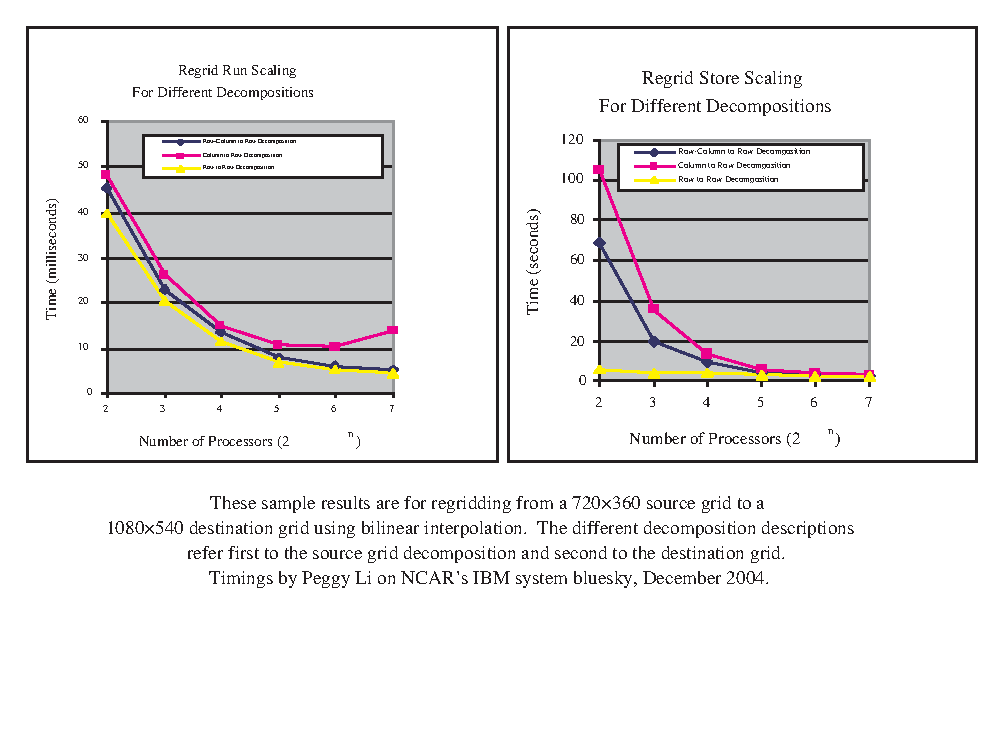
\includegraphics{RegridScaling}}
\caption{Sample scaling graphs for Regrid Run and Store routines. }
\label{fig:RegridScaling}
\end{figure}
\end{center}

\subsubsection{Bilinear Regridding Algorithm}
\label{sec:BilinearRegrid}

     The bilinear regridding method uses a local bilinear approximation
     to interpolate to a point in a quadrilateral grid.  This is applicable
     only for logically-rectangular or block-structured logically-rectangular
     grids.  Standard bilinear interpolation schemes can be found in many textbooks.
     Here we present a more general scheme which uses a local bilinear approximation
     to interpolate to a point in a quadrilateral grid.  Consider the grid points
     shown in Figure~\ref{fig:quad} labelled with logically-rectangular indices
     (e.g. $(i,j)$).

\begin{figure}
\caption{A general quadrilateral grid. \label{fig:quad}}
\begin{picture}(10,10)

\put(1.0,1.0){\line(2,1){5.0}}
\put(6.0,3.5){\line(1,2){2.5}}
\put(1.0,1.0){\line(1,2){2.5}}
\put(3.5,6.0){\line(2,1){5.0}}

\put(1.0,1.0){\circle*{0.1}}
\put(6.0,3.5){\circle*{0.1}}
\put(3.5,6.0){\circle*{0.1}}
\put(8.5,8.5){\circle*{0.1}}
\put(5.25,5.0){\circle*{0.1}}

\put(0.75,0.5 ){1 $(i,j)$}
\put(6.25,3.25){2 $(i+1,j)$}
\put(1.75,6.0 ){$(i,j+1)$ 4}
\put(8.75,8.5 ){3 $(i+1,j+1)$}
\put(5.0 ,5.0 ){$P$}

\end{picture}
\end{figure}

     Let the latitude-longitude coordinates of point 1 be $(\theta(i,j),\phi(i,j))$,
     the coordinates of point 2 be $(\theta(i+1,j),\phi(i+1,j))$, etc. 
     Now let $\alpha$ and $\beta$ be
     continuous local coordinates such that the coordinates $(\alpha,\beta)$
     of point 1 are $(0,0)$, point 2 are $(1,0)$, point 3 are $(1,1)$ and
     point 4 are $(0,1)$.  If point $P$ lies inside the cell formed by the four
     points above, the function $f$ at point $P$ can be approximated by
\begin{eqnarray}\label{eq:bilinear}
f_P & = & (1-\alpha)(1-\beta)f(i,j) + \alpha(1-\beta)f(i+1,j) + \nonumber \\
    &   & \alpha\beta f(i+1,j+1) + (1-\alpha)\beta f(i,j+1)  \\
    & = & w_1 f(i,j) + w_2 f(i+1,j) + w_3 f(i+1,j+1) + w_4 f(i,j+1). \nonumber
\end{eqnarray}

     The remapping weights must therefore be computed by finding $\alpha$ and
     $\beta$ at point $P$.  

     The latitude-longitude coordinates $(\theta,\phi)$ of point $P$ are known
     and can also be approximated by
\begin{eqnarray}\label{eq:thetaphi}
\theta & = & (1-\alpha)(1-\beta)\theta_1 + \alpha(1-\beta)\theta_2 + \nonumber
          \alpha\beta \theta_3 + (1-\alpha)\beta \theta_4 \\
\phi   & = & (1-\alpha)(1-\beta)\phi_1   + \alpha(1-\beta)\phi_2 +
          \alpha\beta \phi_3 + (1-\alpha)\beta \phi_4.
\end{eqnarray}

     Because (\ref{eq:thetaphi}) is nonlinear in $\alpha$ and $\beta$, we must
     linearize and iterate toward a solution.  Differentiating 
     (\ref{eq:thetaphi}) results in
\begin{equation}
\left[\begin{array}{c} \delta\theta \\ \delta\phi \end{array}\right] = A
\left[\begin{array}{c} \delta\alpha \\ \delta\beta \end{array}\right],
\end{equation}

     where

\begin{equation}
A = \left[\begin{array}{cc}
(\theta_2-\theta_1) + (\theta_1-\theta_4+\theta_3-\theta_2)\beta &
(\theta_4-\theta_1) + (\theta_1-\theta_4+\theta_3-\theta_2)\alpha \\
(\phi_2-\phi_1) + (\phi_1-\phi_4+\phi_3-\phi_2)\beta &
(\phi_4-\phi_1) + (\phi_1-\phi_4+\phi_3-\phi_2)\alpha
\end{array}\right].
\end{equation}

     Inverting this system,

\begin{equation}\label{eq:dalpha}
\delta\alpha = \left|\begin{array}{cc}
\delta\theta &
(\theta_4-\theta_1) + (\theta_1-\theta_4+\theta_3-\theta_2)\alpha \\
\delta\phi &
(\phi_4-\phi_1) + (\phi_1-\phi_4+\phi_3-\phi_2)\alpha 
\end{array}\right| \div \det(A),
\end{equation}

     and

\begin{equation}\label{eq:dbeta}
\delta\beta = \left|\begin{array}{cc}
(\theta_2-\theta_1) + (\theta_1-\theta_4+\theta_3-\theta_2)\beta &
\delta\theta \\
(\phi_2-\phi_1) + (\phi_1-\phi_4+\phi_3-\phi_2)\beta &
\delta\phi 
\end{array}\right| \div \det(A).
\end{equation}

     Starting with an initial guess for $\alpha$ and $\beta$ (say 
     $\alpha=\beta=0$), equations~(\ref{eq:dalpha}) and (\ref{eq:dbeta})
     can be iterated until $\delta\alpha$ and $\delta\beta$ are suitably small.
     The weights can then be computed from (\ref{eq:bilinear}).  Note that
     for simple latitude-longitude grids, this iteration will converge in the
     first iteration.

     In order to compute the weights using this general bilinear iteration,
     it must be determined in which box the point $P$ resides.  Because this
     method is valid only for logically-rectangular grids, the sweep algorithm
     can be optimized to take advantage of this restriction.  The sweep
     method currently in ESMF steps through each data point $P$ on the destination
     grid.  For each destination point, it then loops through the cells on the
     source grid, comparing the coordinates of point $P$ with the bounding box
     formed by each cell's minimum and maximum coordinates.  Most source cells can
     be efficiently eliminated from the sweep via this simple test.  This loop is
     further optimized by tracking the index of the source cell containing the
     previous point and using that as the initial starting index for the next
     point's sweep, since both grids are logically ordered.  Please see
     Figure~\ref{fig:BilinearSweep} for an illustration of the sweep algorithm.

\begin{center}
\begin{figure}
\scalebox{0.9}{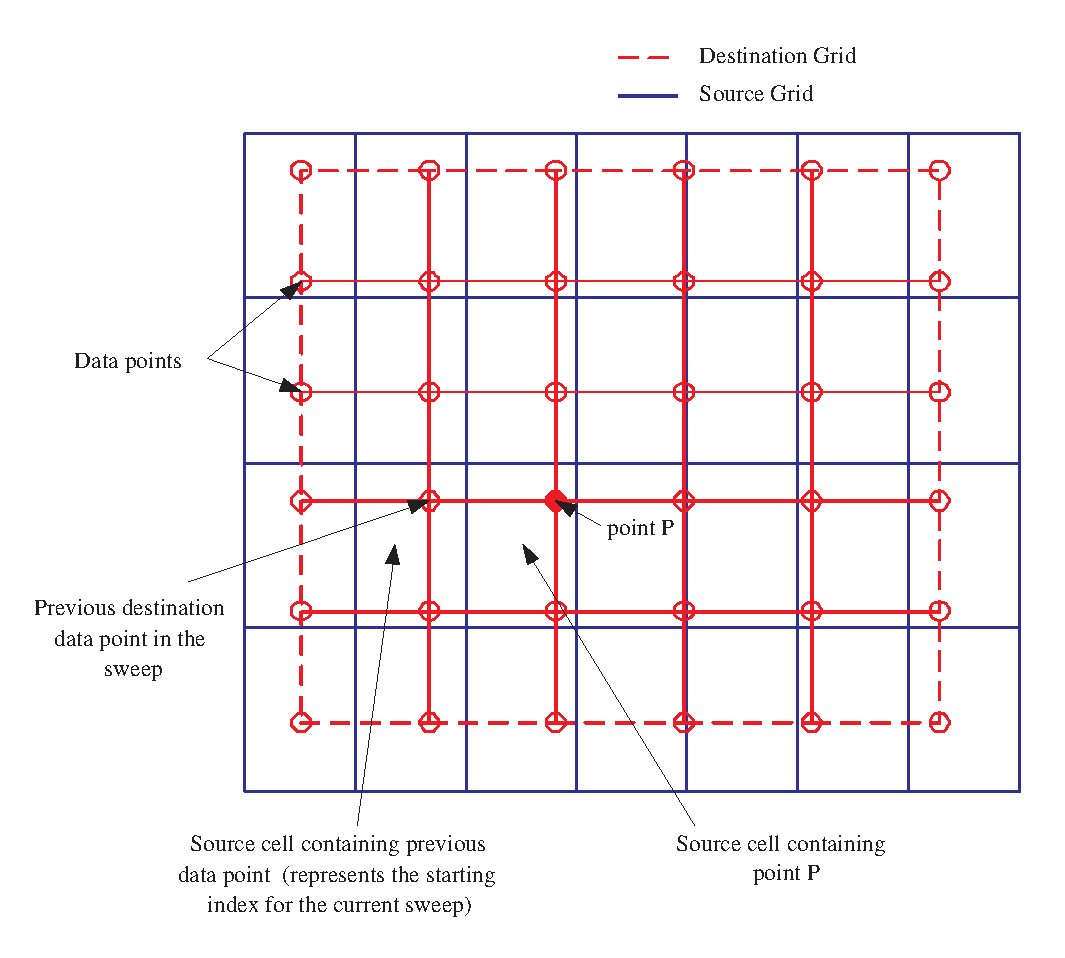
\includegraphics{BilinearSweep}}
\caption{Illustration of the Bilinear Sweep Algorithm. }
\label{fig:BilinearSweep}

\end{figure}
\end{center}

\subsubsection{Bicubic Regridding Algorithm}  Not yet implemented!
\label{sec:BicubicRegrid}

     Like the bilinear remapping, bicubic remapping is applicable
     only for logically-rectangular or block-structured logically-rectangular
     grids.  The bicubic remapping exactly follows the bilinear remapping except
     that four weights for each corner point are required.  Thus, num\_wts
     is set to four for this option.  The bicubic remapping is

\begin{eqnarray}\label{eq:bicubic}
f_P & = & 
    (1 - \beta^2(3-2\beta))(1 - \alpha^2(3-2\alpha))f(i  ,j  ) + \nonumber \\
& & (1 - \beta^2(3-2\beta))     \alpha^2(3-2\alpha) f(i+1,j  ) + \nonumber \\
& &      \beta^2(3-2\beta)      \alpha^2(3-2\alpha) f(i+1,j+1) + \nonumber \\
& &      \beta^2(3-2\beta) (1 - \alpha^2(3-2\alpha))f(i  ,j+1) + \nonumber \\
& & (1 - \beta^2(3-2\beta))\alpha  (\alpha-1)^2 
                        {{\partial f}\over{\partial i}}(i  ,j  ) + \nonumber \\
& & (1 - \beta^2(3-2\beta))\alpha^2(\alpha-1) 
                        {{\partial f}\over{\partial i}}(i+1,j  ) + \nonumber \\
& &      \beta^2(3-2\beta) \alpha^2(\alpha-1)
                        {{\partial f}\over{\partial i}}(i+1,j+1) + \nonumber \\
& &      \beta^2(3-2\beta) \alpha  (\alpha-1)^2 
                        {{\partial f}\over{\partial i}}(i  ,j+1) + \nonumber \\
& & \beta  (\beta-1)^2(1 - \alpha^2(3-2\alpha))
                        {{\partial f}\over{\partial j}}(i  ,j  ) + \nonumber \\
& & \beta  (\beta-1)^2     \alpha^2(3-2\alpha) 
                        {{\partial f}\over{\partial j}}(i+1,j  ) + \nonumber \\
& & \beta^2(\beta-1)       \alpha^2(3-2\alpha)
                        {{\partial f}\over{\partial j}}(i+1,j+1) + \nonumber \\
& & \beta^2(\beta-1)  (1 - \alpha^2(3-2\alpha)) 
                        {{\partial f}\over{\partial j}}(i  ,j+1) + \nonumber \\
& & \alpha  (\alpha-1)^2\beta  (\beta-1)^2
           {{\partial^2 f}\over{\partial i \partial j}}(i  ,j  ) + \nonumber \\
& & \alpha^2(\alpha-1)  \beta  (\beta-1)^2 
           {{\partial^2 f}\over{\partial i \partial j}}(i+1,j  ) + \nonumber \\
& & \alpha^2(\alpha-1)  \beta^2(\beta-1)
           {{\partial^2 f}\over{\partial i \partial j}}(i+1,j+1) + \nonumber \\
& & \alpha  (\alpha-1)^2\beta^2(\beta-1)
           {{\partial^2 f}\over{\partial i \partial j}}(i  ,j+1)
\end{eqnarray}

     where $\alpha$ and $\beta$ are identical to those found in the bilinear
     case and are found using an identical algorithm.  Note that unlike the
     conservative remappings, the gradients here are gradients with respect to
     the {\em logical} variable and not latitude or longitude.  Lastly, the four
     weights corresponding to each address pair correspond to the weight
     multiplying the field value at the point, the weight multiplying the
     gradient with respect to $i$, the weight multiplying the gradient with
     respect to $j$, and the weight multiplying the cross gradient in that order.


\subsubsection{Conservative Regridding Algorithms}
\label{sec:ConserveRegrid}

     First-order and second-order conservative remapping share a common
     algorithm, though currently only first-order has been implemented.
     ESMF implements a conservative remapping scheme described in detail
     elsewhere \cite{Jones1999}.  A brief outline will be given
     here to aid the user in understanding this regridding algorithm.

     To compute a flux on a new (destination) grid which results in the same
     energy or water exchange as a flux $f$ on an old (source) grid, the
     destination flux $F$ at a destination grid cell $k$ must satisfy

\begin{equation}\label{eq:local}
\overline{F}_k = {1\over{A_k}}\int\int_{A_k} fdA,
\end{equation}

     where $\overline{F}$ is the area-averaged flux and $A_k$ is the area of
     cell $k$. Because the integral in (\ref{eq:local}) is over the area of 
     the destination grid cell, only those cells on the source grid that are
     covered at least partly by the destination grid cell contribute to the
     value of the flux on the destination grid.  If cell $k$ overlaps $N$ cells
     on the source grid, the remapping can be written as 

\begin{equation}\label{eq:rmpsum}
\overline{F}_k = 
{1\over{A_k}} \sum_{n=1}^N \int\int_{A_{nk}} f_ndA,
\end{equation}

     where $A_{nk}$ is the area of the source grid cell $n$ covered by the
     destination grid cell $k$, and $f_n$ is the local value of the flux in the
     source grid cell (see Figure~\ref{fig:grids}).  Note that (\ref{eq:rmpsum})
     is normalized by the destination area $A_k$ corresponding to the
     {\tt ESMF\_RegridNormOpt} value of {\tt ESMF\_REGRID\_NORM\_DSTAREA}.  The
     sum of the weights for a destination cell $k$ in this case would be between
     0 and 1 and would be the area fraction if $f_n$ were identically 1 
     everywhere on the source grid.  The normalization option
     {\tt ESMF\_REGRID\_NORM\_FRACAREA} would actually divide by the area of the
     source grid overlapped by cell $k$: 

\begin{equation}
\sum_{n=1}^N \int\int_{A_{nk}}dA.
\end{equation}

     For this normalization option, remapping a function $f$ which is 1
     everywhere on the source grid would result in a function $F$ that is
     exactly one wherever the destination grid overlaps a non-masked source
     grid cell and zero otherwise.  A normalization option of
     {\tt ESMF\_REGRID\_NORM\_NONE} would result in the actual angular area
     participating in the remapping.

     Assuming $f_n$ is constant across a source grid cell, (\ref{eq:rmpsum})
     would lead to the first-order area-weighted schemes used in current coupled
     models.  A more accurate form of the remapping is obtained by using 

\begin{equation}\label{eq:gradient}
f_n = \overline{f}_n + 
                   \nabla_n f\cdot({\vec{r}} - \vec{r}_n),
\end{equation}

     where $\nabla_n f$ is the gradient of the flux in cell $n$ and $\vec{r}_n$
     is the centroid of cell $n$ defined by

 \begin{equation}\label{eq:centroid}
\vec{r}_n = {1\over{A_n}}\int\int_{A_n}\vec{r}dA.
\end{equation}

     Such a distribution satisfies the conservation constraint and is equivalent
     to the first terms of a Taylor series expansion of $f$ around $\vec{r}_n$.
     The remapping is thus second-order accurate if $\nabla_n f$ is at least a 
     first-order approximation to the gradient.

     The remapping can now be expanded in spherical coordinates as 

\begin{equation}\label{eq:remap}
\overline{F}_k = \sum_{n=1}^{N} \left[\overline{f}_n w_{1nk} + 
\left({{\partial f}\over{\partial \theta}}\right)_n w_{2nk} +
\left({1\over{\cos\theta}}{{\partial f}\over{\partial \phi}}\right)_n w_{3nk}
\right],
\end{equation}

     where $\theta$ is latitude, $\phi$ is longitude and the three remapping
     weights are

\begin{equation}\label{eq:weights1}
w_{1nk} = {1\over{A_k}}\int\int_{A_{nk}}dA, \\
\end{equation}
\begin{eqnarray}\label{eq:weights2}
w_{2nk} & = & {1\over{A_k}}\int\int_{A_{nk}}(\theta-\theta_n)dA \nonumber \\
        & = & {1\over{A_k}}\int\int_{A_{nk}}\theta dA -
              {{w_{1nk}}\over{A_n}}\int\int_{A_n}\theta dA,
\end{eqnarray}

     and

\begin{eqnarray}\label{eq:weights3}
w_{3nk} & = & {1\over{A_k}}\int\int_{A_{nk}}\cos\theta(\phi-\phi_n)dA \nonumber \\
        & = & {1\over{A_k}}\int\int_{A_{nk}}\phi\cos\theta dA -
              {{w_{1nk}}\over{A_n}}\int\int_{A_n}\phi\cos\theta dA .
\end{eqnarray}

     Again, if the gradient is zero, ({\ref{eq:remap}}) reduces to a first-order
     area-weighted remapping. 

     The area integrals in equations~(\ref{eq:weights1})--(\ref{eq:weights3})
     are computed by converting the area integrals into line integrals using the
     divergence theorem.  Computing line integrals around the overlap regions
     is much simpler; one simply integrates first around every grid cell on the
     source grid, keeping track of intersections with destination grid lines,
     and then one integrates around every grid cell on the destination grid in
     a similar manner.  After the sweep of each grid, all overlap regions have
     been integrated.

     Choosing appropriate functions for the divergence, the integrals in
     equations~(\ref{eq:weights1})--(\ref{eq:weights3}) become

\begin{equation}
\int\int_{A_{nk}}dA = \oint_{C_{nk}} -\sin\theta d\phi,
\end{equation}
\begin{equation}
\int\int_{A_{nk}}\theta dA = 
 \oint_{C_{nk}} [-\cos\theta-\theta\sin\theta]d\phi,
\end{equation}
\begin{equation}
\int\int_{A_{nk}}\phi\cos\theta dA = 
\oint_{C_{nk}} -{\phi\over 2}[\sin\theta\cos\theta + \theta]d\phi,
\end{equation}

     where $C_{nk}$ is the counterclockwise path around the region $A_{nk}$.
     Computing these three line integrals during the sweeps of each grid
     provides all the information necessary for computing the remapping weights.

\begin{figure}
  \caption{An example of a triangular destination grid cell $k$ overlapping
           a quadrilateral source grid.  The region $A_{kn}$
           is where cell $k$ overlaps the quadrilateral cell $n$.
           Vectors used by search and intersection routines are
           also labelled. \label{fig:grids}}

\begin{picture}(10,10)

\put(2.5 ,0   ){\line(2,1){7.5}}
\put(1.25,2.5 ){\line(2,1){7.5}}
\put(0   ,5.0 ){\line(2,1){7.5}}
%\put(0   ,3.75){\line(2,1){10.0}}

\put(  0,5.0 ){\line(1,-2){2.5}}
\put(2.5,6.25){\line(1,-2){2.5}}
\put(5.0,7.5 ){\line(1,-2){2.5}}
\put(7.5,8.75){\line(1,-2){2.5}}

\put(1.25,3.125){\line(1,0){5.0}}
\put(6.25,3.125){\line(1,4){1.0}}
{\thicklines
\put(7.25,7.125){\vector(-3,-2){6.0}}
\put(5.0 ,7.5  ){\vector(1,-2){1.25}}
%\put(5.0 ,7.5  ){\vector(6,-1){2.25}}
\put(5.0 ,7.5  ){\vector(4,-1){2.25}}
}

\put(6.25 ,7.375){$\vec{r}_{1b}$}
\put(4.875,6.75 ){$\vec{r}_{12}$}
\put(4.375,5.625){$\vec{r}_{be}$}

\put(4.25 ,7.75 ){$(\theta_1,\phi_1)$}
\put(6.375,5.0  ){$(\theta_2,\phi_2)$}
\put(7.5  ,7.125){$(\theta_b,\phi_b)$}
\put(0.25 ,3.125){$(\theta_e,\phi_e)$}

\put(5.0 ,7.5  ){\circle*{0.1}}
\put(6.25,5.0  ){\circle*{0.1}}
\put(7.25,7.125){\circle*{0.1}}
\put(1.25,3.125){\circle*{0.1}}

\put(5.625,5.625){Cell $k$}
\put(6.25 ,2.5  ){Cell $n$}
\put(5.0  ,3.75 ){$A_{kn}$}

\end{picture}
\end{figure}

     As described above, the algorithm for computing the remapping weights
     is relatively simple.  The process amounts to finding the location of
     the endpoint of a segment and then finding the next intersection with
     the other grid.  The line integrals are then computed and summed according
     to which grid cells are associated with that particular subsegment.  The
     most time-consuming portion of the algorithm is finding which cell on one
     grid contains an endpoint from the other grid.  This process consists
     of sweeping through lists of cells from the other grid, hunting for
     intersections with an identified subsegment.   Much of the potential for
     optimization of regridding algorithms comes from limiting the range of
     cells to sweep.  Optimal methods can be more easily written when the grid
     is well structured and regular.  However, for a general grid, a hierarchy
     of methods appears to work best.  In the ESMF
     implementation, two algorithms are used to restrict the range of cells
     that are swept.  First, prior to looping through the cells on either grid,
     coordinate bins are created from the other grid.  In this process, the local
     physical domain of the grid being swept is divided into logical blocks, each
     one represented by a bin.  The cells of the grid being swept are looped through
     to determine the minimum and maximum grid indices corresponding to each bin's
     range of physical coordinates.  Each bin therefore identifies an index range
     corresponding to a physical coordinate range.  Then when the sweep begins,
     only those cells in the index range belonging to the same coordinate bin as
     the identifed subsegment are used.  Please reference
     Figure~\ref{fig:ConservSweep} for an illustration of binning and the sweep
     algorithm.

\begin{center}
\begin{figure}
\scalebox{0.9}{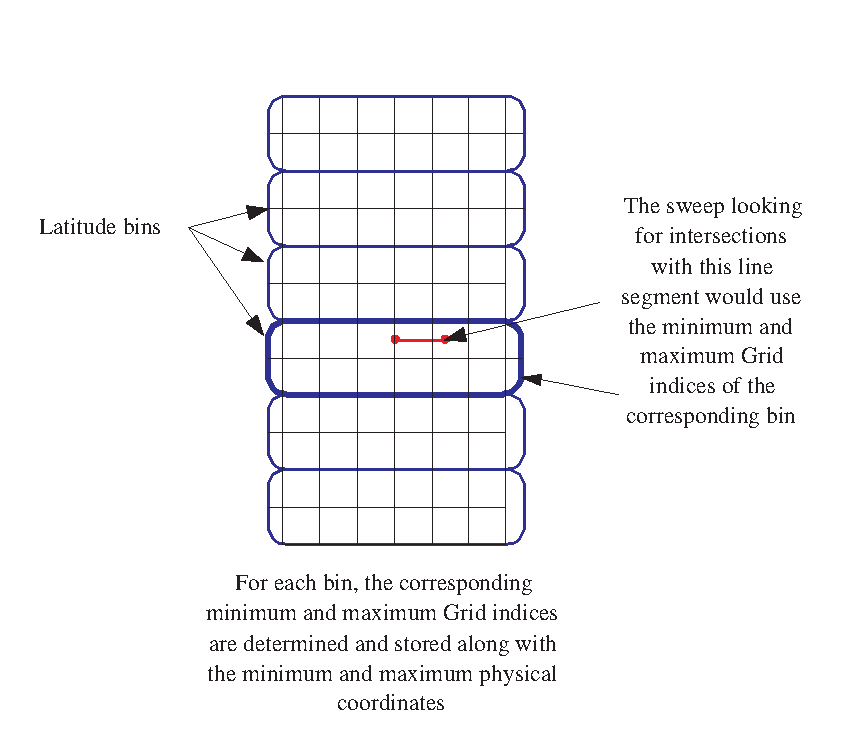
\includegraphics{ConservSweep}}
\caption{Illustration of the Conservative Sweep Algorithm. }
\label{fig:ConservSweep}
\end{figure}
\end{center}

     Note that currently ESMF creates bins based
     only on coordinates in the second grid direction (typically "y" or "latitude").
     The second stage checks the bounding box of each grid cell in the determined
     bin.  The bounding box is formed by the cell's minimum and maximum coordinates.
     This process further restricts the actual sweep to a small number of cells.

     Once the sweep has been restricted, a robust algorithm that works for most
     cases is a cross-product test.  In this test, a cross product is computed
     between the vector corresponding to a cell side ($\vec{r}_{12}$ in
     Figure~\ref{fig:grids}) and a vector extending from the beginning of the
     cell side to the search point ($\vec{r}_{1b}$).  If 

\begin{equation}\label{eq:cross}
\vec{r}_{12} \times \vec{r}_{1b} > 0,
\end{equation}

     the point lies to the left of the cell side.  If (\ref{eq:cross}) holds for
     every cell side, the point is enclosed by the cell.  This test is not
     completely robust and will fail for grid cells that are non-convex.

% \subsubsection{Intersections}\label{sec:intersect}

     Once the location of an initial endpoint is found, it is necessary to check
     to see if the segment intersects with the cell side.  If the segment is
     parametrized as
\begin{eqnarray}
\theta &=& \theta_b + s_1 (\theta_e - \theta_b) \nonumber \\
\phi   &=& \phi_b + s_1 (\phi_e - \phi_b) 
\end{eqnarray}
     and the cell side as
\begin{eqnarray}
\theta &=& \theta_1 + s_2 (\theta_2 - \theta_1) \nonumber \\
\phi   &=& \phi_1 + s_2 (\phi_2 - \phi_1),
\end{eqnarray}
     where $\theta_1, \phi_1, \theta_2, \phi_2, \theta_b,$ and $\theta_e$ are
     endpoints as shown in Figure~\ref{fig:grids}, the intersection of the two
     lines occurs when $\theta$ and $\phi$ are equal.  The linear system 
\begin{equation}
\left[ \begin{array}{cc} 
(\theta_e - \theta_b) & (\theta_1 - \theta_2) \\
(\phi_e - \phi_b) & (\phi_1 - \phi_2) \\
\end{array} \right]
\left[ \begin{array}{c} s_1 \\ s_2 \\ \end{array} \right] = 
\left[ \begin{array}{c} 
(\theta_1 - \theta_b) \\ (\phi_1 - \phi_b)  \\
\end{array} \right]
\end{equation}
     is then solved to determine $s_1$ and $s_2$ at the intersection point.  If
     $s_1$ and $s_2$ are between zero and one, an intersection occurs with that
     cell side. 

     It is important also to compute identical intersections during the sweeps
     of each grid.  To ensure that this will occur, the entire line segment is
     used to compute intersections rather than using a previous or next
     intersection as an endpoint.

% \subsubsection{Coincidences}

     Often, pairs of grids will share common lines (e.g. the Equator).  When
     this is the case, the method described above will double-count the
     contribution of these line segments.  Coincidences can be detected when
     computing cross products for the search algorithm described above.  If
     the cross product is zero in this case, the endpoint lies on the cell
     side.  A second cross product between the line segment and the cell side
     can then be computed.  If the second cross product is also zero, the
     lines are coincident.  Once a coincidence has been detected, the
     contribution of the coincident segment can be computed during the
     first sweep and ignored during the second sweep.

% \subsubsection{Spherical coordinates}\label{sec-sphere}

     Some aspects of the spherical coordinate system introduce additional
     problems for the method described above.  Longitude is multiple valued
     on one line on the sphere, and this branch cut may be chosen differently
     by different grids.  Care must be taken when calculating intersections 
     and line integrals to ensure that the proper longitude values are used.
     A simple method is to always check to make sure the longitude is in the
     same interval as the source grid cell center.

     Another problem with computing weights in spherical coordinates is the
     treatment of the pole.  First, note that although the pole is physically
     a point, it is a line in latitude-longitude space and has a nonzero
     contribution to the weight integrals.  If a grid does not contain the
     pole explicitly as a grid vertex, the pole contribution must be added
     to the appropriate cells.  The pole contribution can be computed analytically.

     The pole also creates problems for the search and intersection algorithms
     described above.  For example, a grid cell that overlaps the pole can
     result in a nonconvex cell in latitude-longitude coordinates.  The
     cross-product test described above will fail in this case.  In addition,
     segments near the pole typically exhibit large changes in longitude even
     for very short segments.  In such a case, the linear parametrizations used
     above result in inaccuracies for determining the correct intersections.

     To avoid these problems, a coordinate transformation can be used poleward
     of a given threshold latitude (typically within one degree of the pole).
     A possible transformation is the Lambert equivalent azimuthal projection
\begin{eqnarray}
X &=& 2\sin\left({\pi \over 4} - {\theta \over 2}\right)\cos\phi \nonumber \\
Y &=& 2\sin\left({\pi \over 4} - {\theta \over 2}\right)\sin\phi 
\end{eqnarray}
     for the North Pole.  The transformation for the South Pole is similar.
     This transformation is only used to compute intersections; line integrals
     are still computed in latitude-longitude coordinates.  Because intersections
     computed in the transformed coordinates can be different from those computed
     in latitude-longitude coordinates, line segments which cross the latitude
     threshold must be treated carefully.  To compute the intersections
     consistently for such a segment, intersections with the threshold latitude
     are detected and used as a normal grid intersection to provide a clean break
     between the two coordinate systems.

\subsubsection{Overview of Parallelization of Regrid}
On parallel processing platforms, the physical domains of the source and
destination Grids are decomposed into logical Decomposition Elements (DEs), as
illustrated in Figure~\ref{fig:ParallelRegrid}.  In order to calculate
interpolation weights, each destination DE will require coordinate
data from any of the source Grid that
overlaps it in physical space, which may span several DEs from the source Grid.
Corresponding source Field data is necessary later for regridding calculations
using the regridding weights.  The DEs for each Grid are mapped to sets of PETs,
which can be either shared or unique.  However, RegridStore and Regrid must
be called with a VM encompassing the union of the sets of PETS, typically from
a CouplerComponent.  In any case, most situations will require data transfer
between PETs for regridding.  Once source data is available locally, the
regridding algorithms discussed earlier can be applied.

\begin{center}
\begin{figure}
\scalebox{0.9}{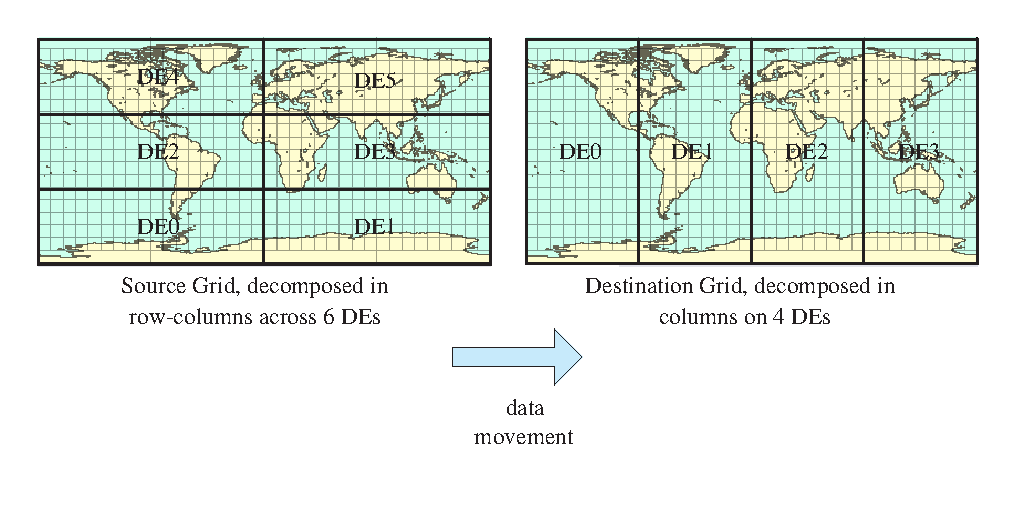
\includegraphics{ParallelRegrid}}
\caption{Illustration of Parallel Regridding. }
\label{fig:ParallelRegrid}
\end{figure}
\end{center}

There are four major sections of regridding that are impacted by the
parallelization process: identifying necessary data, transferring that data, the
sweep algorithms, and then calculating and applying the interpolation weights to
calculate regridded Fields.  Each will be discussed below.

\subsubsection{Parallelization of Regrid: Identification of Necessary Data}

The calculation of interpolation weights requires coordinate information from
both source and destination Grids, and the application of those weights to
determine regridded values needs corresponding source data.  In a serial
implementation of regridding, the complete source and destination Grids, with
all their related data, are stored on a single processor.  In a parallel
implementation, the Grids and their corresponding data have been decomposed as
DEs on a number of PETs.  In this situation, none of the PETs responsible for
part of the destination Grid, represented as a DE, necessarily has all the source
data needed for the calculation or application of interpolation weights.  The
easiest approach to making the necessary source information available is to
simply transfer or maintain copies of all of the source Grid coordinate and Field
data on each of those PETs.  However, this tends to be inefficient in terms of
either communication or memory usage, and computational time spent in search
algorithms.  It requires only a slight bit more work to identify which source DEs
intersect the the local destination DE in physical space and then transfer all
the data from those DEs.  In some cases, this will save communication and memory
overhead.  But in other cases, like between one Grid decomposed in rows and
another decomposed by columns as illustrated in Figure~\ref{fig:RToCRegrid}, that
still ultimately means copying all of the source Grid to each destination PET.
It often makes more sense to identify and transfer only the data from the
source Grid that is required by the destination DE.  In a parallel environment,
this means determining which source DEs intersect the local destination DE in
physical space, determining the extent of the data on that source DE that must
be transferred, and then gathering it to the local PET.  Both of these
approaches, either identifying the exact extent of the data that must be
communicated or communicating data as entire DEs, are currently implemented in
the framework.  By default the framework will transfer only the necessary data,
and the option is currently not readily available to users but is set internally
in the Grid code using a parameter called "domainOption."

\begin{center}
\begin{figure}
\scalebox{0.9}{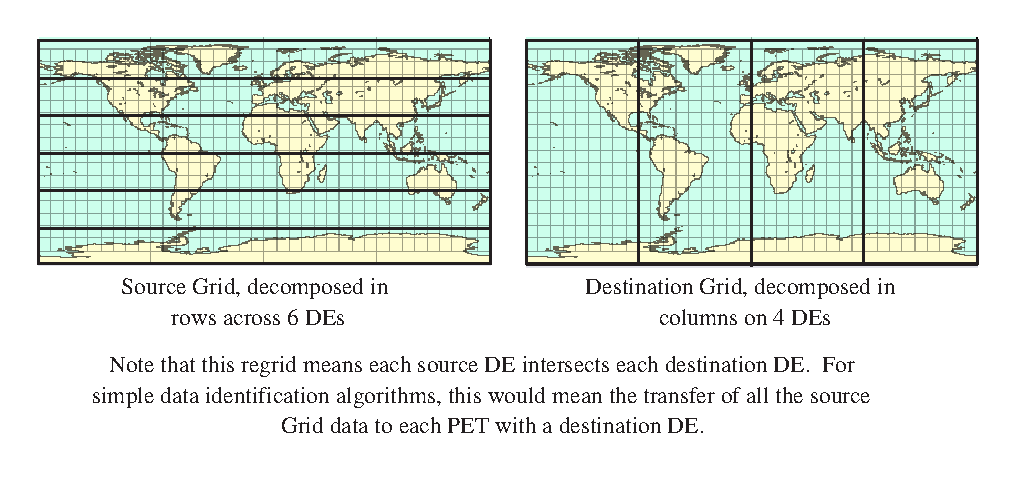
\includegraphics{RToCRegrid}}
\caption{Example of parallel regridding requiring transfer of all data,
         when transferring all data between intersecting DEs. }
\label{fig:RToCRegrid}
\end{figure}
\end{center}

This intersection of DEs is calculated in physical space, using a private Grid
method.  In complicated Grids, these intersections could be non-rectangular, but
for the current logically rectangular Grids each intersection is defined as the
block of the source DE that encompasses any physical overlap with the destination
DE's domain.  Future Grid types would need appropriate methods to identify
intersections, based on their topologies as well as communication issues.  As
shown in Figure~\ref{fig:RegridIntersection}, 
the intersection is often a subset of both the source and destination DEs'
domains, which means that each destination DE must receive and process data from
multiple source DEs.  Each PET involved in a regridding process must calculate
which other PETs it must send data to and how much (if it has a source DE) and
which it must receive data from and how much (if it has a destination DE).  The
current Grid structures contain enough global information to individually
determine the sending data, but the calculation of the data to be received takes
some global communication.

\begin{center}
\begin{figure}
\scalebox{0.9}{\includegraphics{RegridIntersection}}
\caption{Intersection of DE Domains in Parallel Regridding. }
\label{fig:RegridIntersection}
\end{figure}
\end{center}

Regridding algorithms that are point-based (as opposed to cell-based), like
bilinear or bicubic interpolation, require an extra layer of cells around the
identified region, because those algorithms need the location of all surrounding
data points (see Figure~\ref{fig:RegridExtraLayer}).

\begin{center}
\begin{figure} 
\scalebox{0.9}{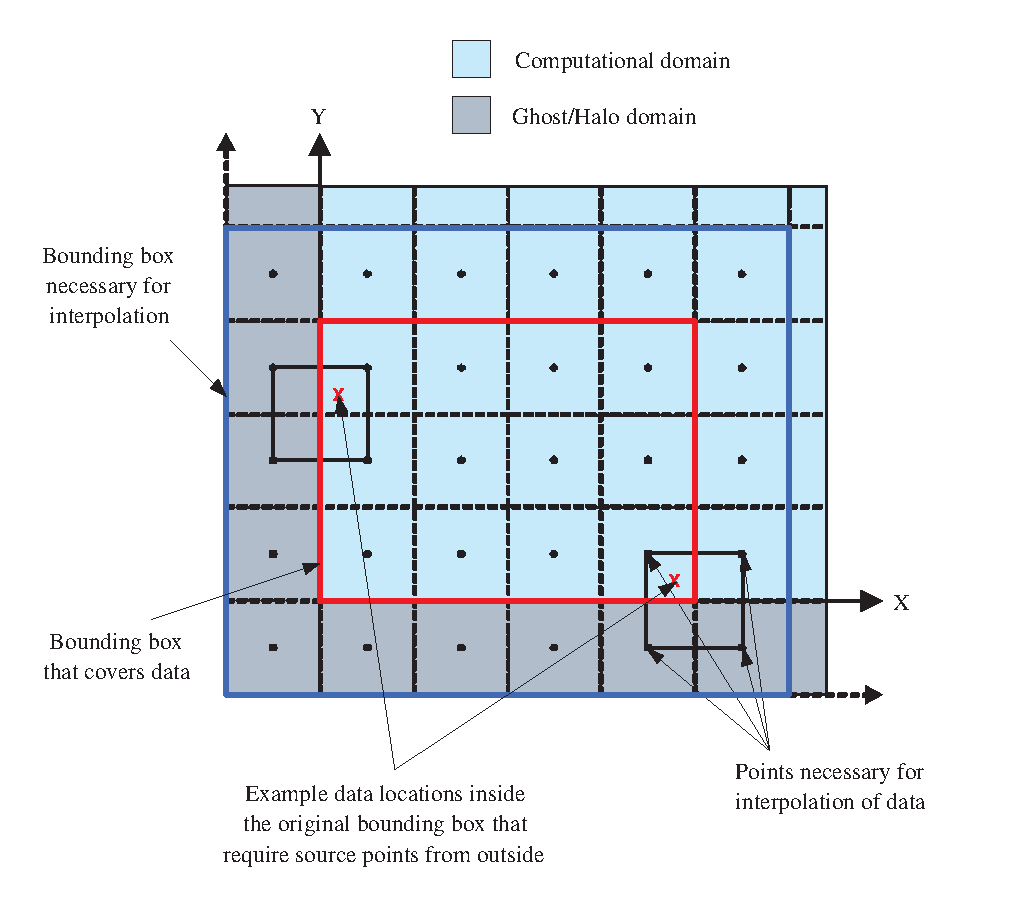
\includegraphics{RegridExtraLayer}}
\caption{Illustration of the extra layer of points required by point-based Regrid
          algorithms. }
\label{fig:RegridExtraLayer}
\end{figure}
\end{center}

Points in this extra layer are assigned internal mask values and are used in the
calculation of interpolation weights for data locations inside the identified
region, but are not assigned weights themselves.  However, these points could be
used in the future as a mechanism for regridding of periodic grids or to avoid
extrapolation issues near the edges of computational grids.

\subsubsection{Parallelization of Regrid: Data Transfer}
Once a block of data to send or receive has been identified, it is stored as an
internal structure called a {\tt domain} and added to a {\tt domainList}.  There
are separate send and receive domainLists for each DE.  From the domainLists,
all the sending and receiving information between PETs is stored internally as a
Route, so that it can leverage other ESMF code for efficient communication.
Internal to the Regrid Store routines, this Route is used to gather necessary
Grid coordinate information.  However, since Routes apply offsets in memory from
a base address rather than addresses themselves, these Routes are reusable by
structures that are distributed in the same way.  The Route to transfer Field
data is similar to that to move Grid coordinates but must be modified for any
Field ranks that do not correspond to a Grid axis and the Field's halo width and
lower bounds.   The modified Route is added to the RouteHandle that is returned
to users and applied later during the routine that actually regrids data from
one Field to another.

Each PET has its own unique Route.  The data it gathers, either Grid coordinates
or Field values, are stored locally as single 1D Arrays.


\subsubsection{Parallelization of Regrid: Sweep Algorithms}
The conservative regrid schemes create coordinate bins to decrease the
number of cells that must be swept, as described earlier.  SCRIP
had an input parameter to set the number of bins to be created, but for a
parallel implementation that number needs to be dynamic.  Dynamic binning
balances the cost, in terms of computational efficiency and storage, of setting
up bins with the savings of having fewer points in each bin to sweep through.  
Rather than specify a number of bins, ESMF added a parameter to set a targeted
number of cells per bin, called {\tt targetBinSize}.  The number of bins on any
PET is set by the local number of cells divided by the targetBinSize.  Currently
this parameter is hard-coded in Regrid, but could be made available to users.
It has been set to 250, based on some preliminary timings on its effect on
Regrid Store (see Figure~\ref{fig:TargetBinSize}).

\begin{center}
\begin{figure}
\scalebox{0.9}{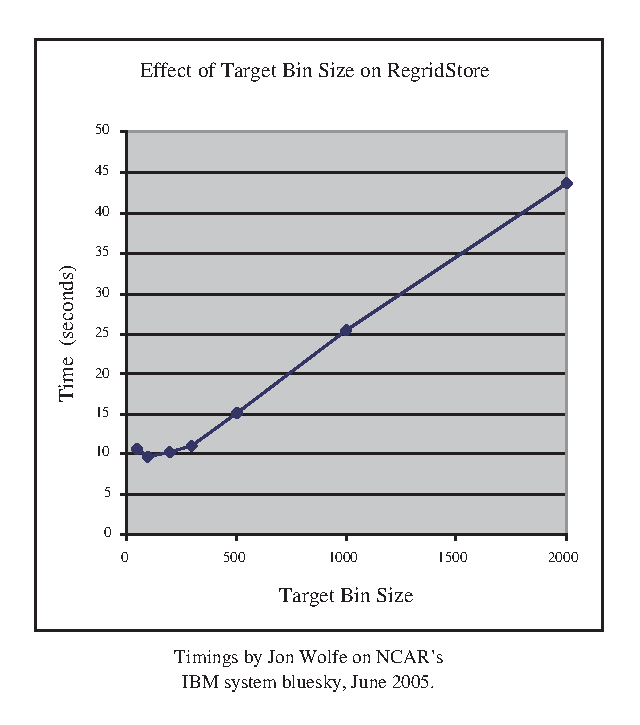
\includegraphics{TargetBinSize}}
\caption{Effect of TargetBinSize on RegridStore timing. }
\label{fig:TargetBinSize}
\end{figure}
\end{center}

Because the conservative regrid algorithm is based on cells and assumes data
values at the vertices, it can operate on the entire set of 1D Arrays of Grid
coordinate information at once.

The bilinear algorithm, on the other hand, is point-based and must assume the
data is logically rectangular.  For that reason, its sweep routine operates on
a single domain at a time, which typically represents just a part of the 1D
gathered Arrays.  It is otherwise unaffected by parallelization.


\subsubsection{Parallelization of Regrid: Calculation and Application of
               Interpolation Weights}

Once the necessary data has been identified and gathered, the calculation and
application of interpolation weights are entirely local operations, requiring no
inter-processor communication.  Once an interpolation weight has been determined
using one of the algorithms described earlier, the weight is stored as part of a
local list of links (described previously) in an object called an
{\tt ESMF\_TransformValues}.  This object is itself part of the 
{\tt ESMF\_RouteHandle} object, and contains:
\begin{description}
   \item [numlist]
         The number of links included in the object.  It also represents the
         size of the corresponding arrays.
   \item [srcindex]
         An array of indices into the local array of source data.
         This array is of size [numlist] and kind ESMF\_KIND\_I4.  Only a single
         integer is required to identify the source index because the source data
         has been gathered as a vector.
   \item [dstindex]
         An array of indices into the local array of destination data.
         This array is of size [2*numlist] and kind ESMF\_KIND\_I4.  Each
         destination index address requires two integers, one for each rank
         of the data array that corresponds to a Grid axis.  However, rather
         than being an array of rank 2, the index pairs are stored sequentially
         in the [dstindex] array.
   \item [weights]
         An array of interpolation weights.  This array is of size [numlist] and
         kind ESMF\_KIND\_R8.
\end{description}
Each link is represented by an entry in this set of arrays.  Also note that there
is a single link for each unique combination of source and destination indices.

The application of the interpolation weights occurs during the Regrid run
routines.  The only necessary communication is that to gather the required source
data locally into a one-dimensional array, using a precomputed Route.
Fundamentally, the application of the weights is a vector multiply of a sparse
matrix, with indirect addressing of the indices.  The main calculation is a loop
over the number of links that effectively sums the product of the source data and
the interpolation weights and loads the result into the corresponding destination
address.  A sample code fragment below illustrates the simplest case, where both
the source and destination data are two-dimensional arrays whose data axes 
correspond to the grids' exactly, with no reordering:

\begin{verbatim}
      do n = 1,numlinks     
        d1 = dstIndex((n-1)*2 + 1)
        d2 = dstIndex((n-1)*2 + 2) 
        s1 = srcIndex(n)           
        dstData2D(d1,d2) = dstData2D(d1,d2) &
                         + (gatheredData(s1) * weights(n))
      enddo  ! numlinks
\end{verbatim}

The coding becomes increasingly more complicated for data arrays of higher rank,
but is inherently similar.



\subsubsection{Regrid Objects}

There is no {\tt ESMF\_Regrid} object per se.  Users are returned an
{\tt ESMF\_RouteHandle} object, which contains one or more {\tt ESMF\_Routes}
used to gather source data, an {\tt ESMF\_TransformValues} object with the
list of links, and an identifier for the type of RouteHandle.  All of these
objects are private and users are not expected to access or modify them.
